% !TEX root = trackjet_intnote.tex

The main quantity of interest here is the charged particle \pt\ distribution in and around the jet as illustrated in Fig.~\ref{Fig:dpt_def}. The measured quantity is defined as:
  \begin{equation}
  \Dptr = \frac{1}{N_{\mathrm{jet}}} \frac{1}{\mathrm{A}} \frac{\mathrm{d} n_{\mathrm{ch}} (\pt, r)}{\mathrm{d} \pt},
%D(\pt,\ptjet) = \frac{1}{N_{\mathrm{jet}}} ~ \frac{1}{\epsilon(\pttrk)} ~ \frac{\mathrm{d} N_{\mathrm{ch}}}{\mathrm{d} \pt}~(\ptjet).
\end{equation}

where $N_{\mathrm{jet}}$ is the number of jets in consideration, $A = \pi (r_{\mathrm{max}}^2 - r_{\mathrm{min}}^2) $ is the area of an annulus around the jet with its inner and outer radii $r_{\mathrm{min}}$ and $r_{\mathrm{max}}$. The angular distance from the jet axis is given by $r = \sqrt{\Delta \eta^2 + \Delta \phi^2}$\footnote{$\Delta \eta$ and $\Delta \phi$ are the distances between the jet axis and the charged particle position in pseudorapidity and azimuth}, and $n_{\mathrm{ch}}(\pt, r)$ is the number of charged particles with a given \pt\ within the annulus. The measurement is performed for the following successive intervals in $r$ around the jet, forming the annuli with inner and outer radii $r_{\textrm{min}}$ and $r_{\textrm{max}}$: 0.0, 0.05, 0.1, 0.15, 0.2, 0.25, 0.3, 0.4, 0.5, 0.6, 0.7, 0.8
%, 0.7, 0.8, 1.0, 1.2.

\begin{figure}
\centerline{
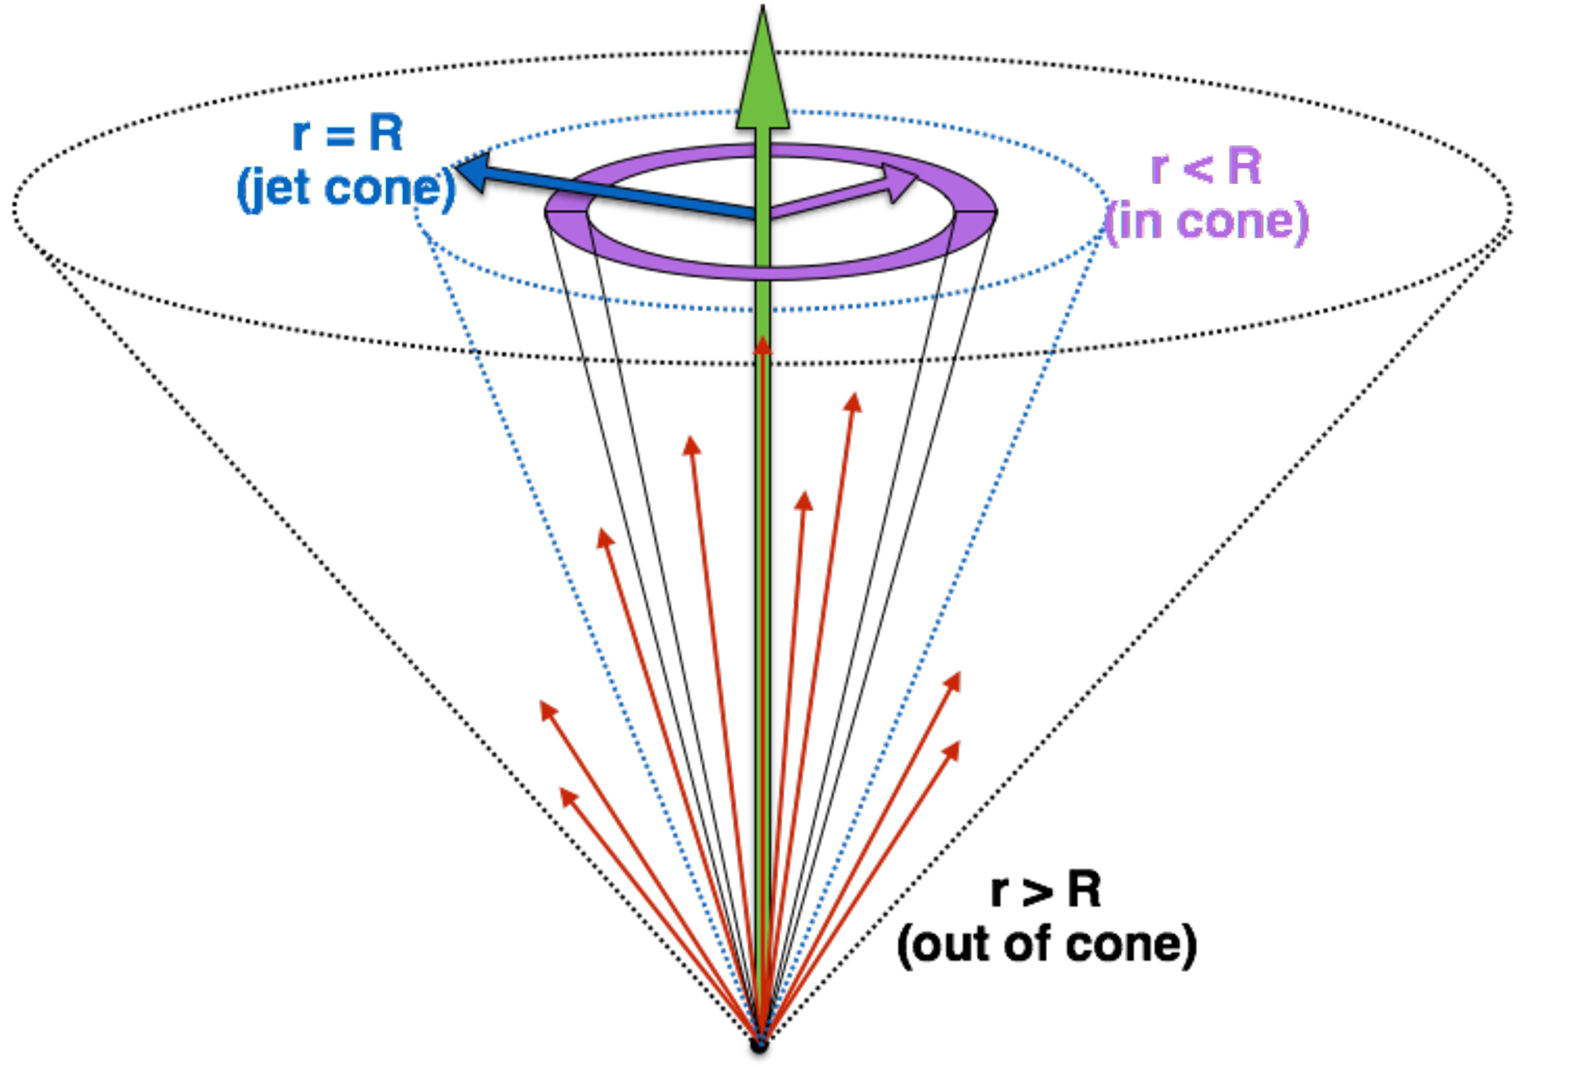
\includegraphics[width=0.55\textwidth]{figures_general/fragScheme_Shape.pdf} }
\caption{Illustration of the tracks in and around the jet. }
\label{Fig:dpt_def}
\end{figure}

%These distributions are of interest because they indicate how the energy of the jet is lost both in and outside the jet in \pbpb\ collisions. Similar measurements have been made by CMS~\cite{CMSPASHIN16020, Chatrchyan:2014ava}, and ATLAS~\cite{ATLAS502FFConf, Aaboud:2017bzv}.

The entire analysis flow of this measurement, along with the various cuts and corrections (discussed in Sec.~\ref{sec:cuts_corrections}) is shown in Fig:\ref{Fig:analysis_flow} and briefly described in the following paragraph.

\begin{figure}
\centerline{
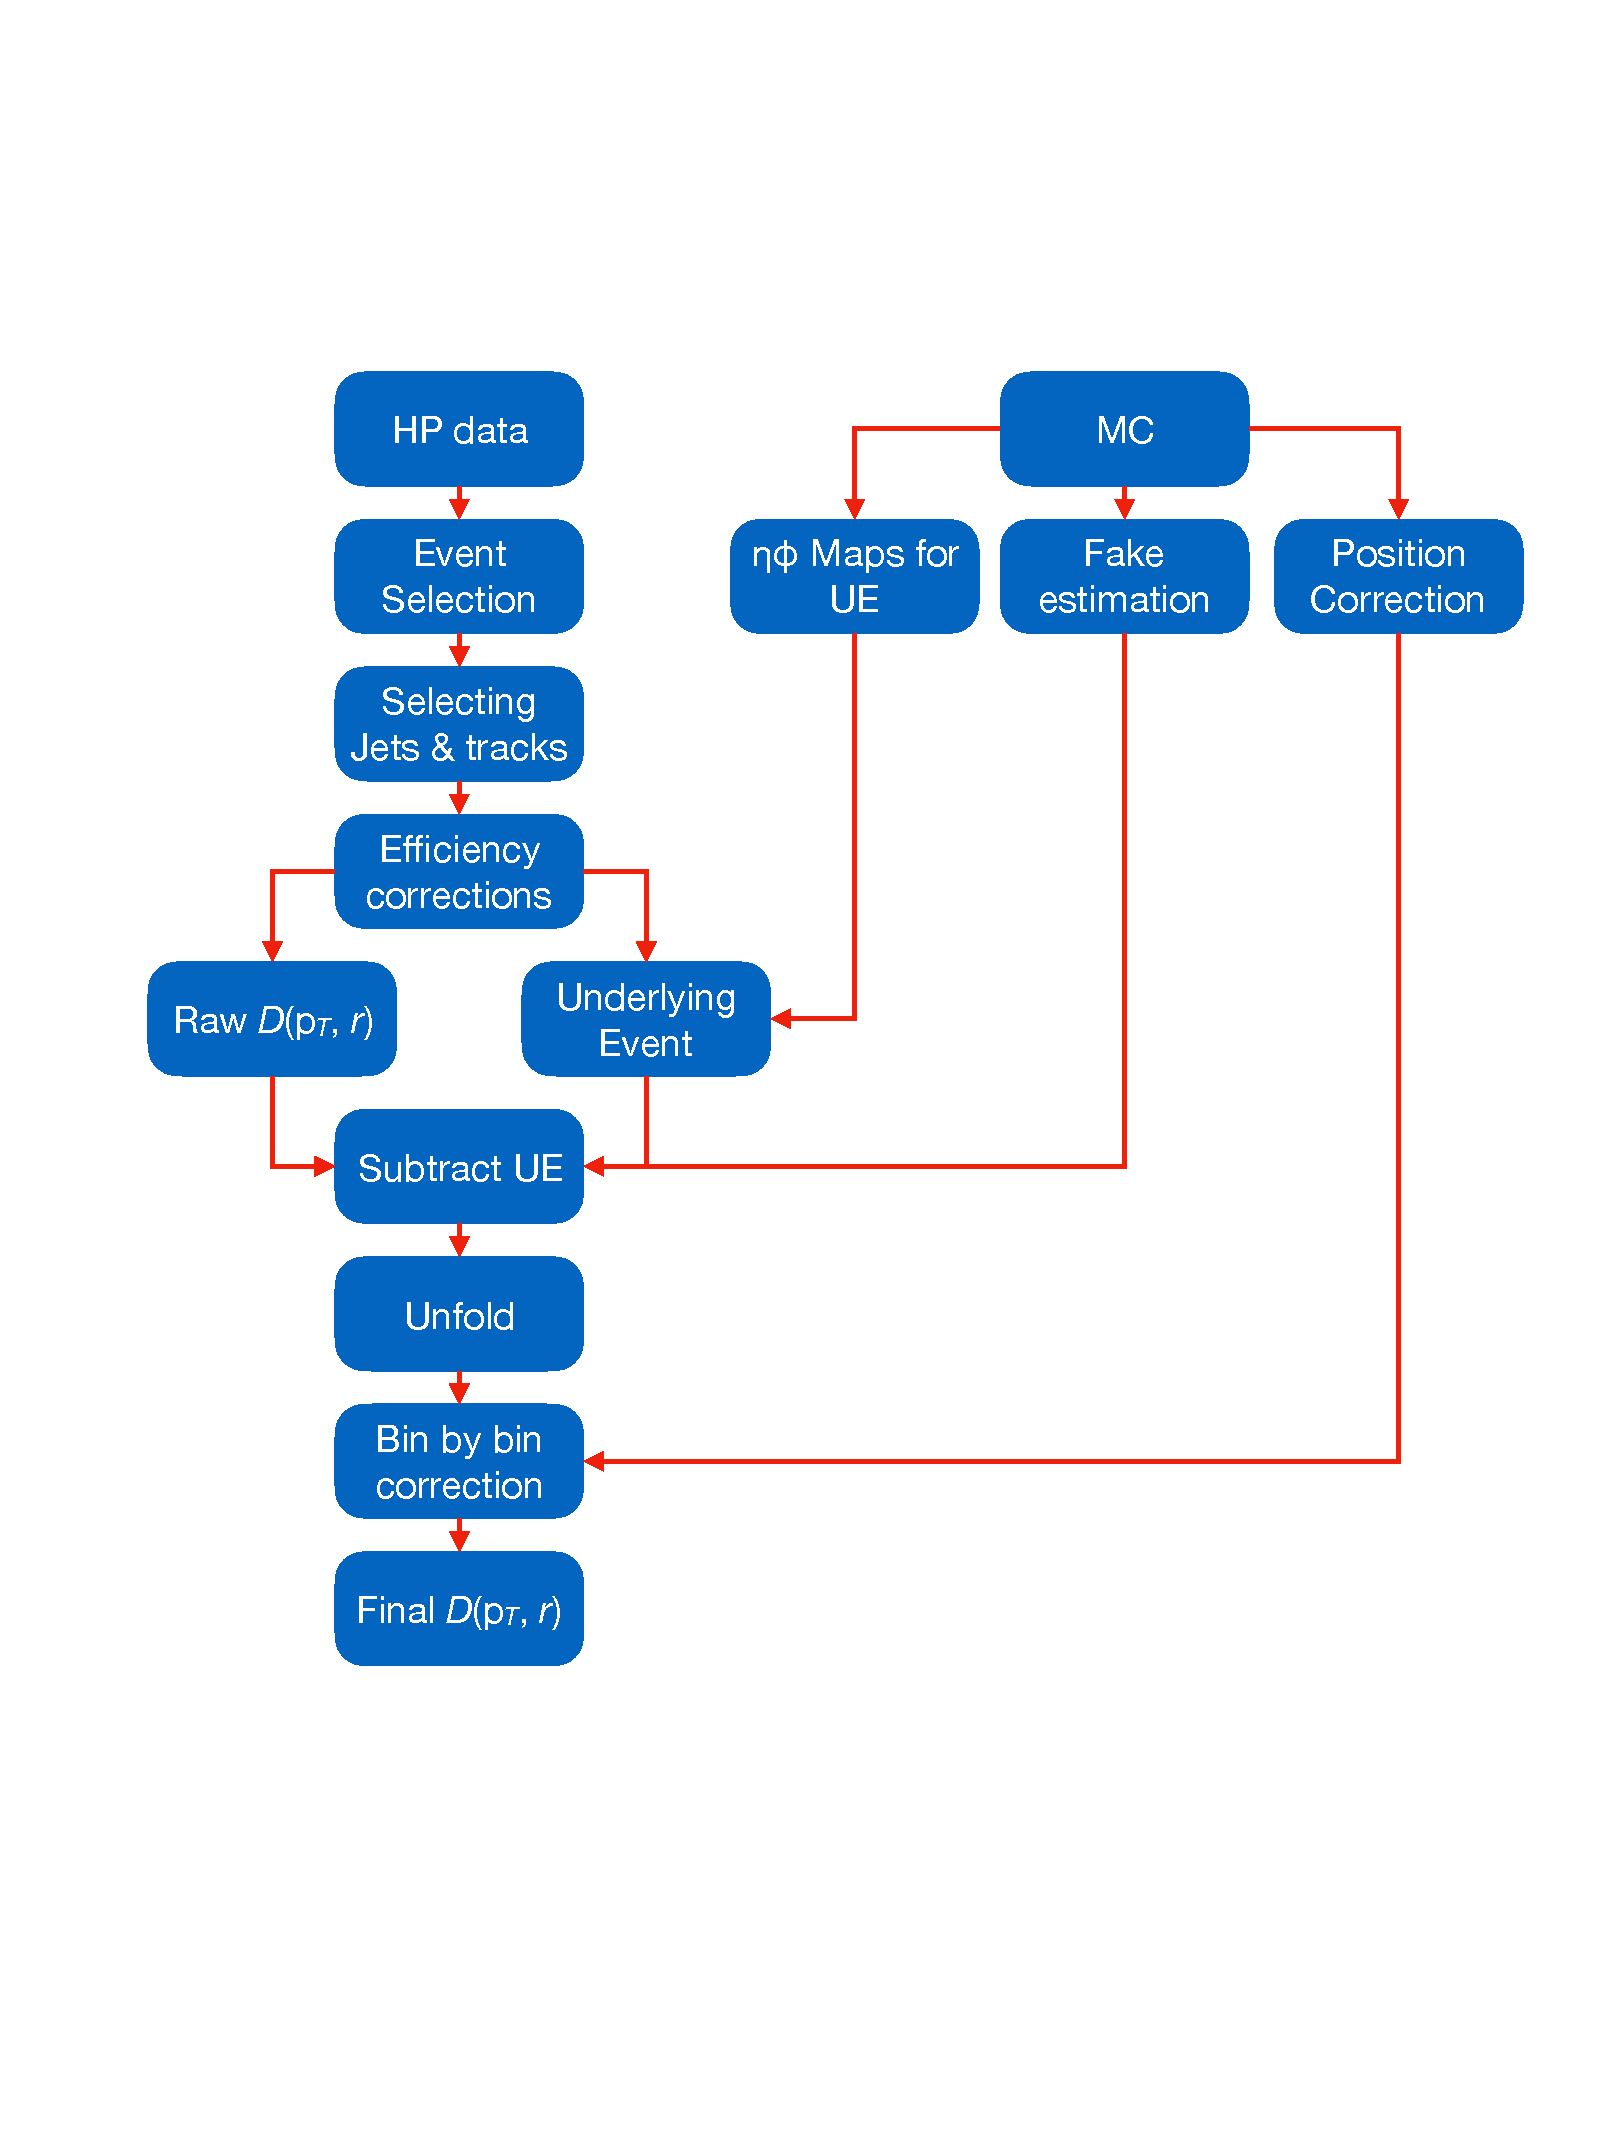
\includegraphics[width=20.cm]{figures_general/Shape_analyses_flow.pdf}
}
\caption{The diagram presents various corrections and cuts that are applied during the analysis.}
\label{Fig:analysis_flow}
\end{figure}

First, the measured charged particle yield, $\text{d}n^{\text{meas}}_{\text{ch}}/\text{d}\pTch$, within an annulus with radii $r_{\text{min}}$ and $r_{\text{max}}$ is evaluated as:
\begin{equation}
\frac{\text{d}n^{\text{meas}}_{\text{ch}}}{\text{d}\pTch} = \frac{1}{\epsilon(\pttrk, \etatrk)} \frac{\Delta N_{\text{ch}} (\pTch, r)}{\Delta \pTch}
\end{equation}

where $\Delta N_{\text{ch}} (\pTch, r)$ is the number of charged particles in a given \pTch\ range that passed the jet and track selection criteria, $r = (r_{\text{min}} + r_{\text{max}}) / 2$, and $\epsilon(\pttrk, \etatrk)$ is the charged particles reconstruction efficiency correction, applied on a track-by-track basis. In \pbpb\ collisions, the measured distributions are affected by charged particles from the underlying event, and thus need to be subtracted out (see Sec.~\ref{sec:cuts_corrections} for details):

\begin{equation}
\frac{\text{d}n^{\text{sub}}_{\text{ch}}}{\text{d}\pTch} = \frac{\text{d}n^{\text{meas}}_{\text{ch}}}{\text{d}\pTch} - \frac{\text{d}n^{\text{UE}}_{\text{ch}}}{\text{d}\pTch}
\end{equation}

The final \Dptr\ distributions are then evaluated after unfolding and normalizing with respect to the unfolded number of jets, $N_{\text{jet}}^{\text{unfolded}}$, as well as the area $A$ of the annulus at given distance $r$ :
\begin{equation}
\Dptr = \frac{1}{N_{\text{jet}}^{\text{unfolded}}} \frac{1}{\text{A}} \frac{\text{d}n^{\text{unfolded}}_{\text{ch}}}{\text{d}\pTch} \quad \quad \text{where } A = \pi (r_{\text{max}}^2 - r_{\text{min}}^2)
\end{equation}

The unfolding procedure is a combination of a two-dimensional Bayesian unfolding method in \ptjet\ and \pttrk, one-dimensional Bayesian unfolding method to correct jet spectra for the normalization and a one-dimensional bin-by-bin correction for the jet and track position resolution. 

The analysis is performed differentially in \ptjet, and centrality, with the jet \pt\ bin size growing logarithmically with \ptjet\ to ensure good statistics in the full range of the measurement. This scheme was also used in other ATLAS jet measurements~\cite{ATLAS276FFConf}. 

In order to quantify the differences between charged particle spectra in \pbpb\ and \pp\  collisions, the ratios of the charged particle spectra in \pbpb\ collisions to those in \pp\ collisions are also reported:
\begin{equation}
   R_{\Dptr} \equiv \frac{\Dptr_{\pbpb}}{\Dptr{\pp}}
\end{equation}
In the absence of modifications to the charged particle spectra in \pbpb\ collisions, both ratios will be unity.


